\documentclass[fontset=windows,12pt]{article}

\usepackage[UTF8]{ctex}
\usepackage[a4paper]{geometry}
\usepackage{amsmath}
\usepackage{fancyhdr}
\usepackage{amsthm}
\usepackage{amssymb}
\usepackage{xcolor}
\usepackage{listings}
\usepackage{graphicx}
\usepackage{circuitikz}
\ctikzset{logic ports=ieee}     %所有逻辑门使用IEEE标准
\usetikzlibrary{calc}           %使用TikZ中的计算功能
\setlength{\headheight}{14.49998pt}

\newtheorem{question}{\hskip 1.7mm \bf}
\renewenvironment{proof}{{\noindent\hskip 2em \bf ֤证明 \quad}}{\hfill$\qed$\par}
\newenvironment{solution}{{\noindent\hskip 2.4em \bf 解 \quad}}

\geometry{left=2.0cm,right=2.0cm,top=2.5cm,bottom=2.5cm}
\begin{document}

\definecolor{CPPLight}  {HTML} {686868}
\definecolor{CPPSteel}  {HTML} {888888}
\definecolor{CPPDark}   {HTML} {262626}
\definecolor{CPPBlue}   {HTML} {4172A3}
\definecolor{CPPGreen}  {HTML} {487818}
\definecolor{CPPBrown}  {HTML} {A07040}
\definecolor{CPPRed}    {HTML} {AD4D3A}
\definecolor{CPPViolet} {HTML} {7040A0}
\definecolor{CPPGray}  {HTML} {B8B8B8}
\lstset{
    columns=fixed,       
    numbers=left,                                        % 在左侧显示行号
    frame=none,                                          % 不显示背景边框
    backgroundcolor=\color[RGB]{245,245,244},            % 设定背景颜色
    keywordstyle=\color[RGB]{40,40,255},                 % 设定关键字颜色
    numberstyle=\footnotesize\color{darkgray},           % 设定行号格式
    commentstyle=\it\color[RGB]{0,96,96},                % 设置代码注释的格式
    stringstyle=\rmfamily\slshape\color[RGB]{128,0,0},   % 设置字符串格式
    showstringspaces=false,                              % 不显示字符串中的空格
    language=c++,                                        % 设置语言
    morekeywords={wire,assign,module,endmodule,always,input,output,alignas,continute,friend,register,true,alignof,decltype,goto,
    reinterpret_cast,try,asm,defult,if,return,typedef,auto,delete,inline,short,
    typeid,bool,do,int,signed,typename,break,double,long,sizeof,union,case,
    dynamic_cast,mutable,static,unsigned,catch,else,namespace,static_assert,using,
    char,enum,new,static_cast,virtual,char16_t,char32_t,explict,noexcept,struct,
    void,export,nullptr,switch,volatile,class,extern,operator,template,wchar_t,
    const,false,private,this,while,constexpr,float,protected,thread_local,xnor,
    const_cast,for,public,throw,std},
    emph={map,set,multimap,multiset,unordered_map,unordered_set,
    unordered_multiset,unordered_multimap,vector,string,list,deque,
    array,stack,forwared_list,iostream,memory,shared_ptr,unique_ptr,
    random,bitset,ostream,istream,cout,cin,endl,move,default_random_engine,
    uniform_int_distribution,iterator,algorithm,functional,bing,numeric,begin,end},
    emphstyle=\color{CPPViolet}, 
}
\newenvironment{correction}{\par\noindent{\color{blue}{\bf{更正\\}}}\quad\color{blue}}{\par}
\pagestyle{fancy}
\lhead{中国科学院大学}
\chead{\bf{2024-25秋数字电路课程}}
\rhead{\emph{2023K8009929044 薛翼舟}}


\begin{center}
\huge{\bf{实验报告1}}
\end{center}

\section{实验目的}
    \subsection{熟悉verilog编程与调试}
    通过编写不同层次的激励文件, 对于多层次结构的程序进行调试
    \subsection{熟悉简单比较器的工作原理}
    \subsection{通过简单模块实例化、连下实现复杂的数字电路}

\section{实验环境}
    AMD Vivado2022.2

\section{原理说明}
    \subsection{4位比较器}
        对于比较器, 采用从高位向地位逐个比较的办法, 如果高位已经比较出结果, 那么低位就不用比较, 逻辑表达式如下
        \begin{align*}
            out\_A\_G\_B &= A_3B'_3+(A_3\odot B_3)A_2B'_2+(A_3\odot B_3)(A_2\odot B_2)A_1B'_1\\
                    &+(A_3\odot B_3)(A_2\odot B_2)(A_1\odot B'_1)A_0B'_0\\
                    &+(A_3\odot B_3)(A_2\odot B_2)(A_1\odot B'_1)(A_0\odot B_0)in\_A\_G\_B\\
            out\_A\_E\_B &=(A_3\odot B_3)(A_2\odot B_2)(A_1\odot B'_1)(A_0\odot B_0)in\_A\_E\_B\\
            out\_A\_L\_B &=(out\_A\_G\_B+out\_A\_E\_B)'
        \end{align*}
    \subsection{16位数值比较器}
        通过将四个4位比较器串行连接起来, 前一个比较器的结果输出是下一个比较器的结果输入, 以此来实现多位比较
    \subsection{4位超前进位加法器}
        直接写出每一个进位的表达式, 进而可以直接输出每一位的结果, 而不用等上一位才能进行下一位, 尽管电路会更为复杂, 
        但是用时会更短, 在超前进位加法器中, 引入了两个新的逻辑变量来简化逻辑表达, 也为实现多位的超前进位加法器提供便利, 逻辑表达式如下
        \begin{align*}
            P_i&=A_i \oplus B_i\\
            G_i&=A_iB_i\\
            CO_i&=G_i+P_i(CI_i)\\
                &=G_i+P_i(G_{i-1}+P_{i-1}(CI_{i-1}))\\
                &=\cdots
        \end{align*}
    \subsection{32位超前进位加法器}
        利用11个4位超前加法器搭建一个32位超前加法器, 形成一个树状结构, 自下而上进行输入之后, 在自上而下计算进位信号等, 最终输出结果
    \subsection{门电路图}
    \begin{figure}[ht]

        \begin{minipage}[t]{0.5\linewidth}  \label{Fig.4}      %图片占用一行宽度的30%
            \centering
            \hspace{2mm}
            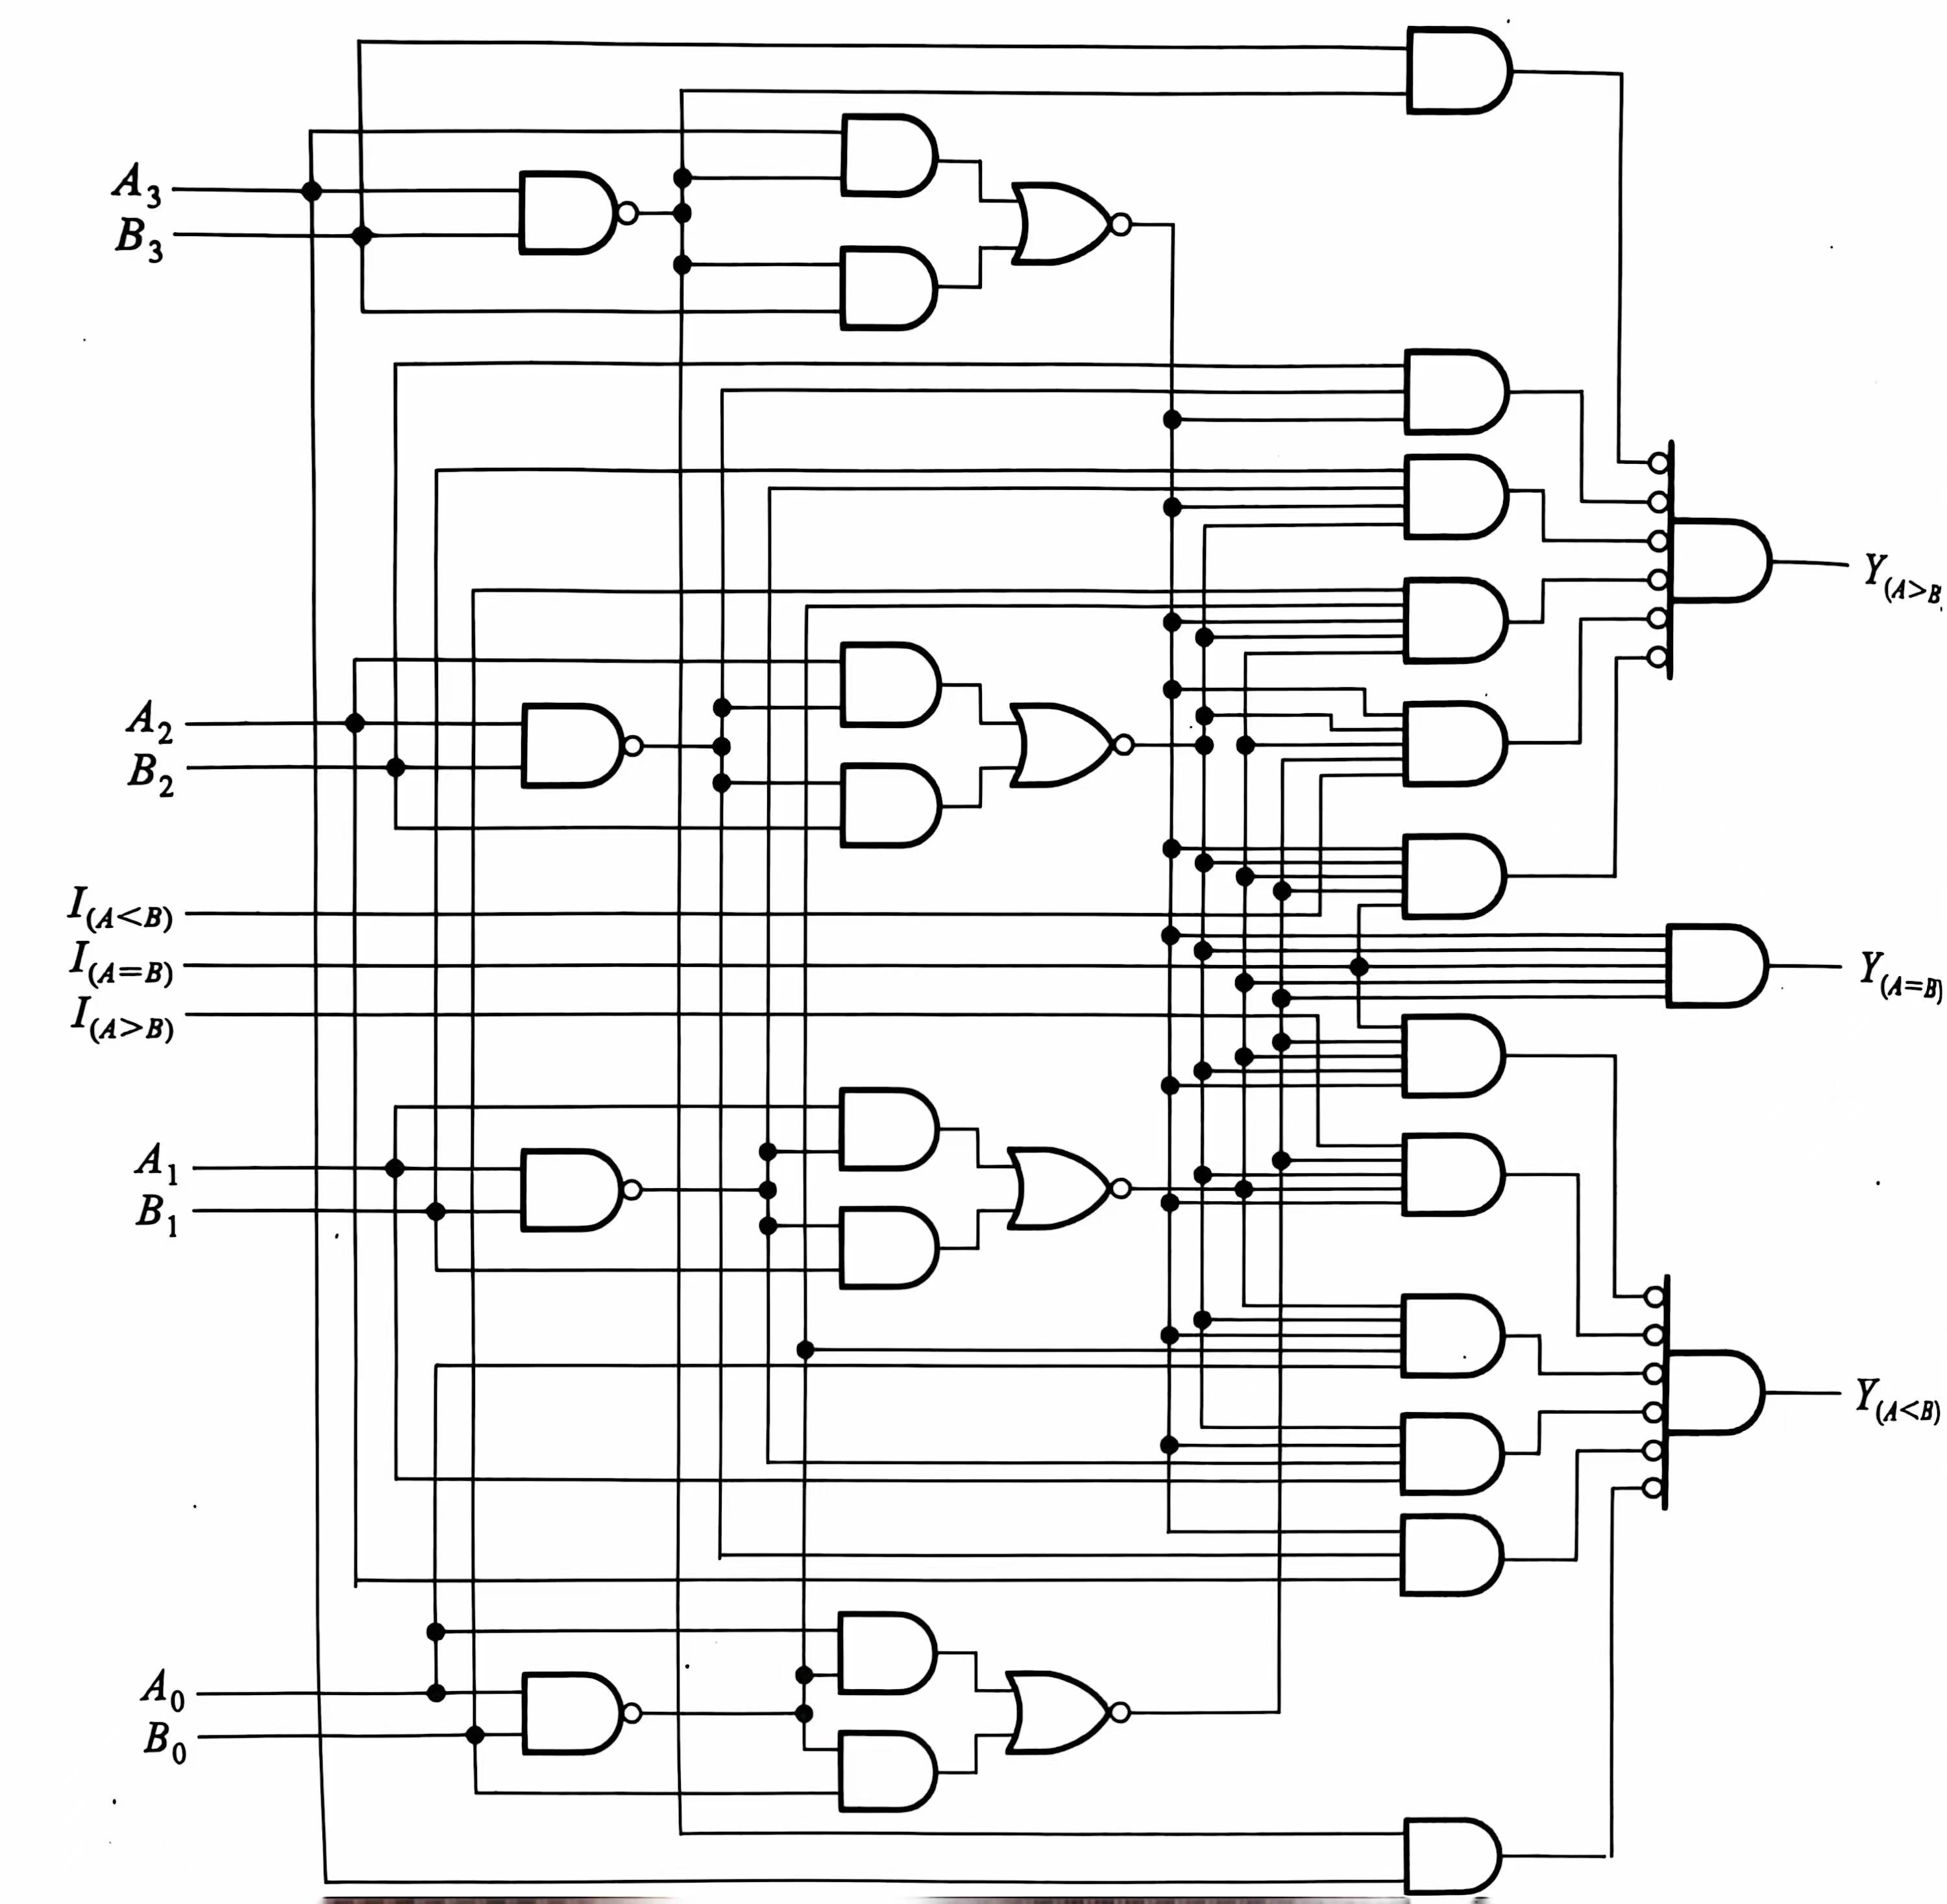
\includegraphics[width=1\textwidth]{4位数值比较器.jpg}
            \caption{4位数值比较器}
        \end{minipage}
        \begin{minipage}[t]{0.5\linewidth}  \label{Fig.4}      %图片占用一行宽度的30%
            \centering
            \hspace{2mm}
            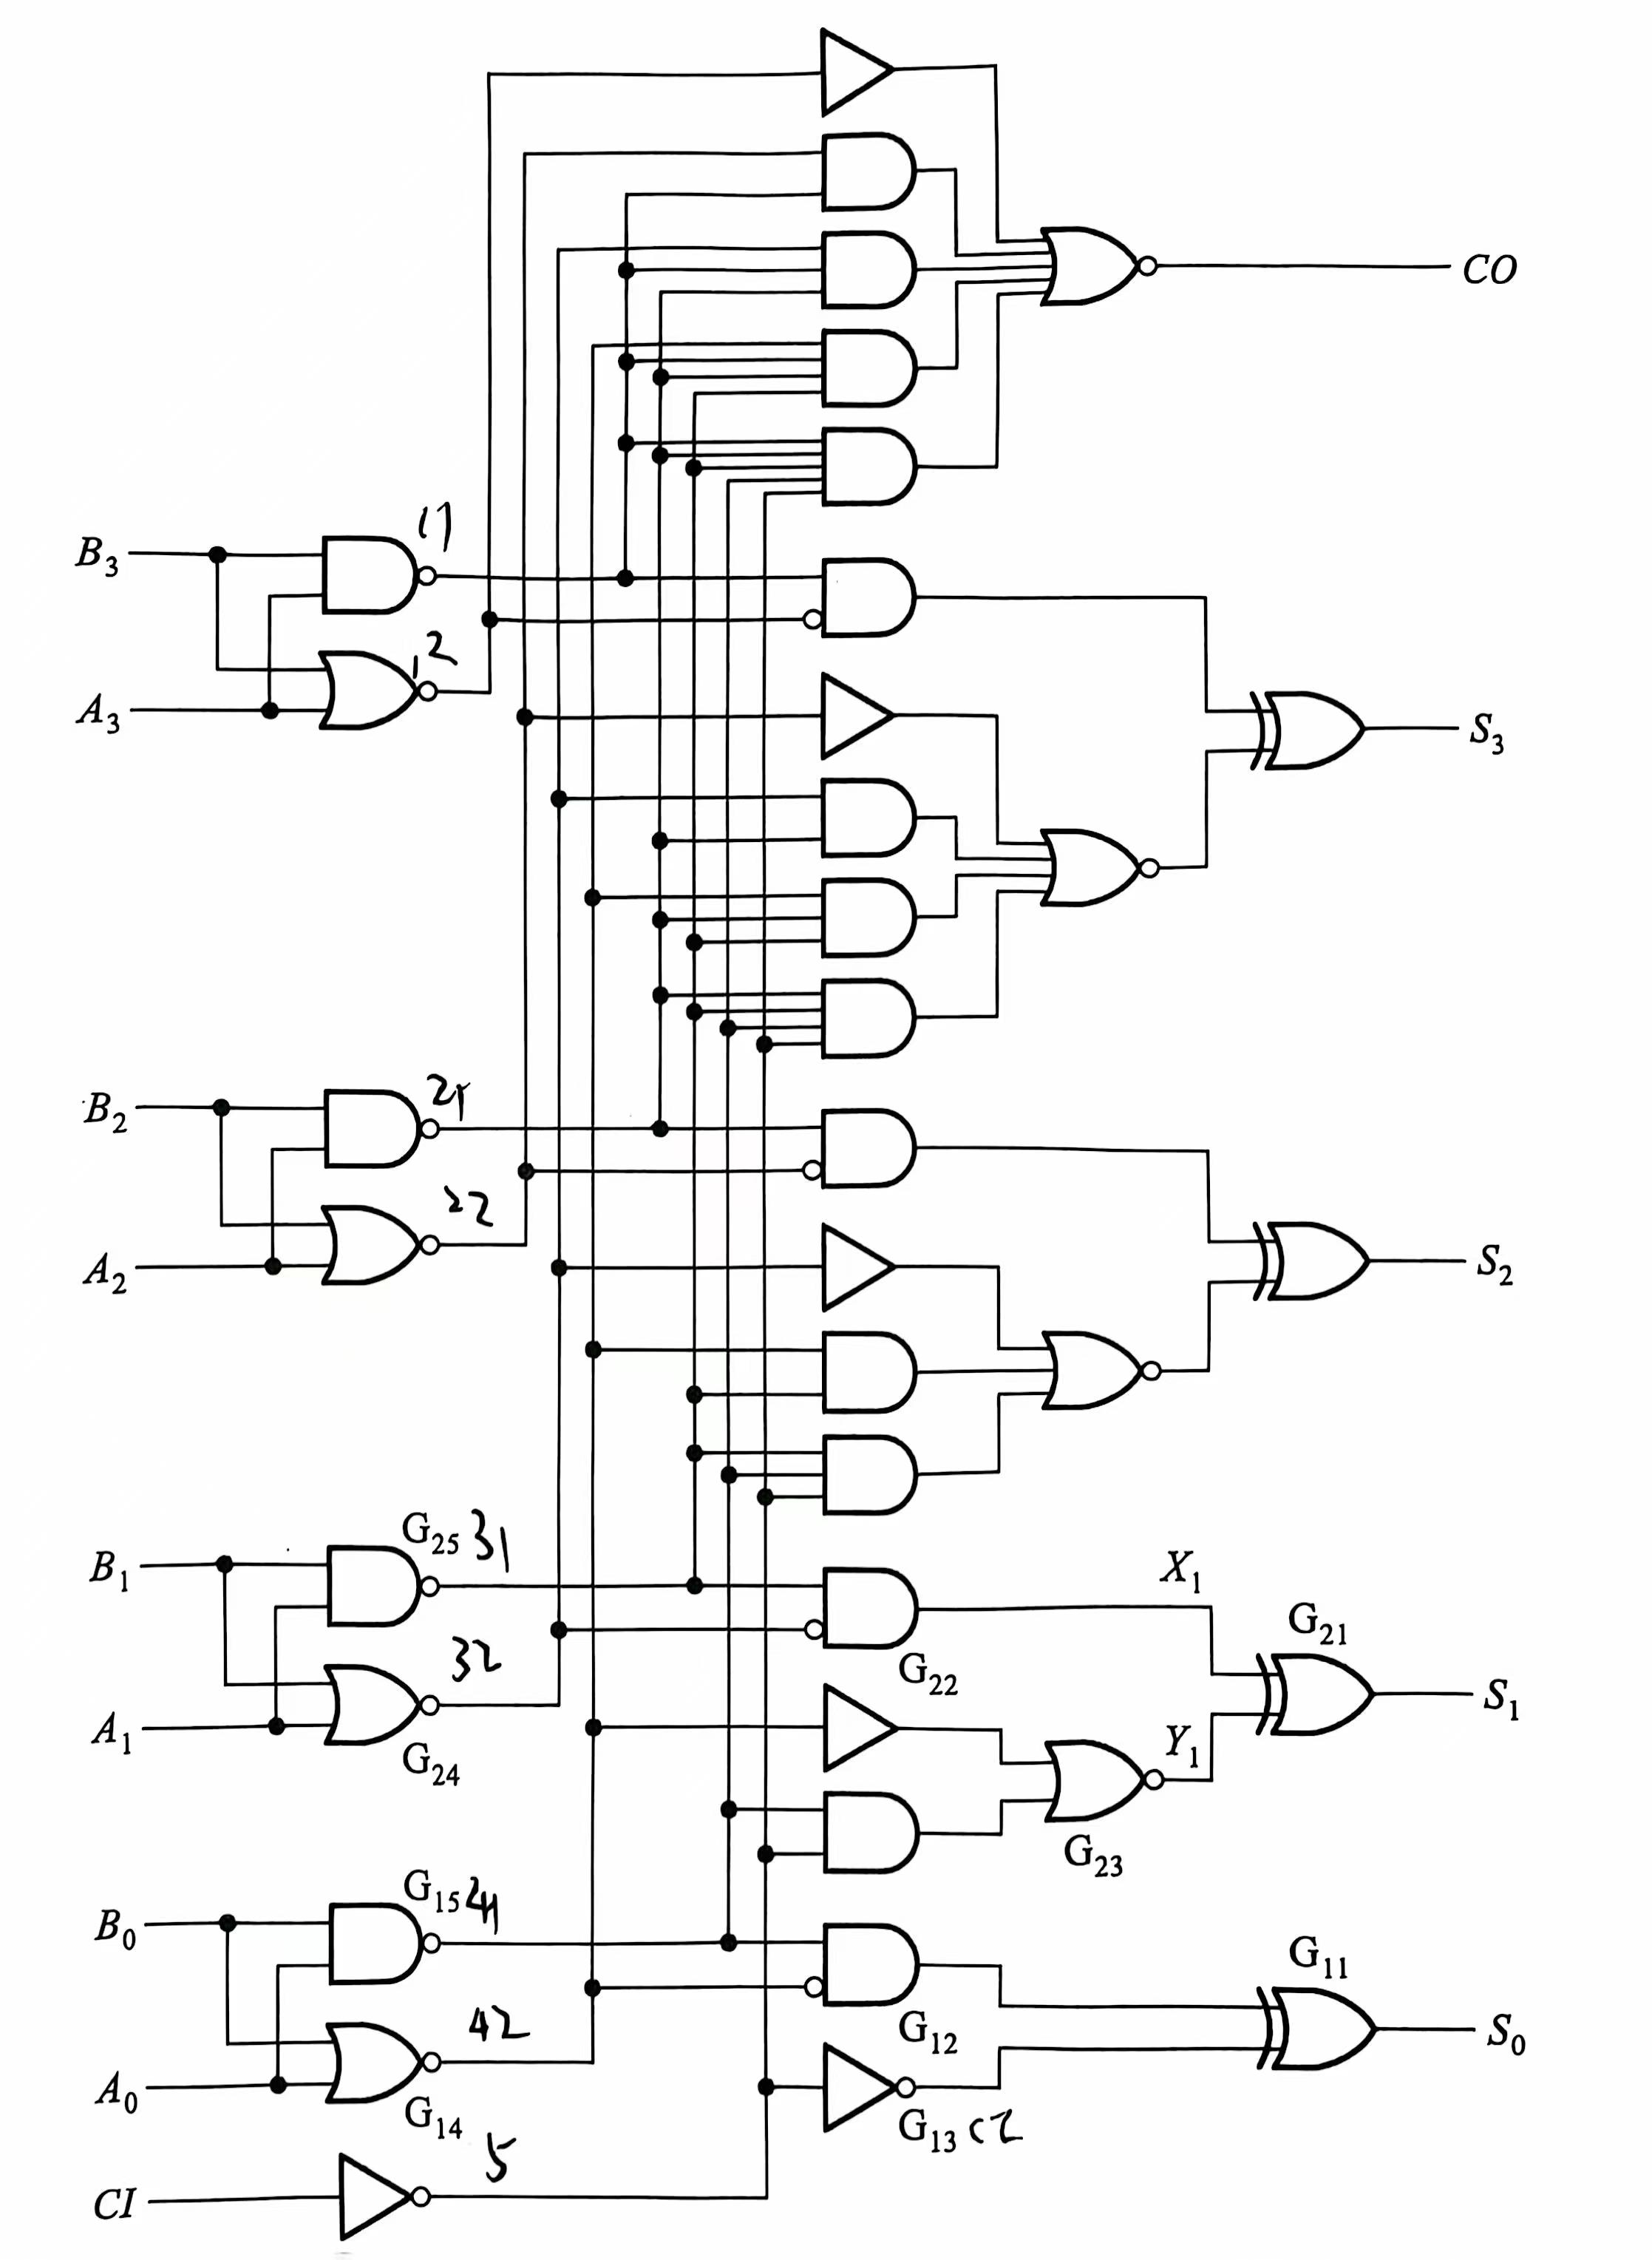
\includegraphics[width=1\textwidth]{4位超前进位加法器`.jpg}
            \caption{4位超前进位加法器}
        \end{minipage}
    \end {figure}


\section{接口定义}
    \subsection{4位数值比较器}
    {\setmainfont{Courier New Bold} 
    \begin{lstlisting}
    module comp_4(
        input [3:0]A,           (4位输入1)
        input [3:0]B,           (4位输入2)
        input in_A_G_B,         (前比较结果A>B输入)
        input in_A_E_B,         (前比较结果A=B输入)
        input in_A_L_B,         (前比较结果A<B输入)
        output reg out_A_G_B,   (比较结果A>B输出)
        output reg out_A_E_B,   (比较结果A=B输出)
        output reg out_A_L_B    (比较结果A<B输出)
    );
    \end{lstlisting}}
    \subsection{16位数值比较器}
        与4位数值比较器的接口定义基本相同, 只是带宽不同, 在此不多赘述

    \subsection{4位超前加法器}
    {\setmainfont{Courier New Bold} 
    \begin{lstlisting}
    module add(
        input [3:0]A,           (4位输入1)
        input [3:0]B,           (4位输入2)
        input Cin,              (进位输入)
        output [3:0]S,          (本位结果输出)
        output [3:0]C,          *(计算中进位输出)
        output Cout,            (进位输出)
        output p,               *(向上层输出p)
        output g                *(向上层输出g)
    );
    \end{lstlisting}}
    值得注意的是, 在这个四位超前加法器中, 有许多接口是为了实现更高位的超前进位加法器定义的, 比如C是用于向下输出
    进位信号的, p和g是向上输出以产生进位信号的, 单纯的四位超前进位加法器并不需要这些端口


\section{调试过程以及结果}
    \subsection{4位和16位数值比较器}
        在编写4位数值比较器时, 唯一遇到的困难是同或的运算如何表示, 经过查询有如下几种表示$S=A\odot B$
        {\setmainfont{Courier New Bold} 
        \begin{lstlisting}
        xnor(S,A,B)
        assign S=(A ^ B)'
        assign S=(A ~^ B)
        \end{lstlisting}}
        波形图如下, check=1表示结果正确
        \begin{figure}[ht]
            \centering
            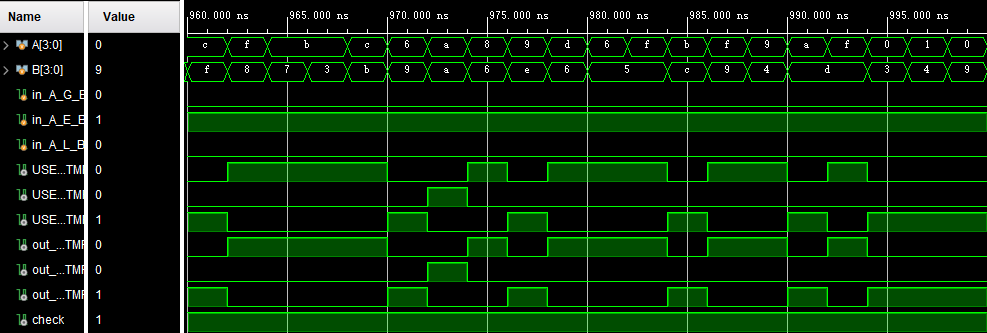
\includegraphics[width=1\textwidth]{4位比较器波形图.jpg}
            \caption{4位数值比较器波形图}
        \end{figure}\par
        \begin{figure}[ht]
            \centering
            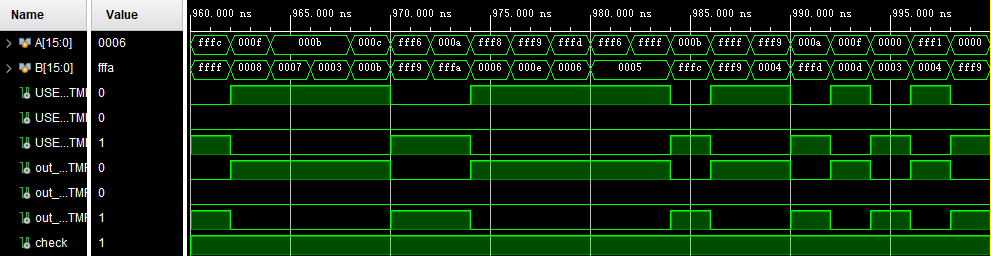
\includegraphics[width=1\textwidth]{16位数值比较器波形图.jpg}
            \caption{16位数值比较器波形图}
        \end{figure}\par

    \subsection{32位超前进位加法器}
        利用4-16-32的结构层层搭建, 形成一个树状结构, 值得注意的是在讲义中最底层向上输出的P和G并不是单纯的P和G, 
        而实际上是如下表达式
        \begin{align*}
            P&=P_3P_2P_1P_0\\
            G&=G_3+P_3G_2+P_3P_2G_1+P_3P_2P_1G_0
        \end{align*}
        采用的主要原理是自下而上输入P、G, 计算出所有进位信号后转而向下输出, 最终计算出结果\\
        本实验中对三个层次都进行了测试, 波形图如下
        \begin{figure}[ht]
            \centering
            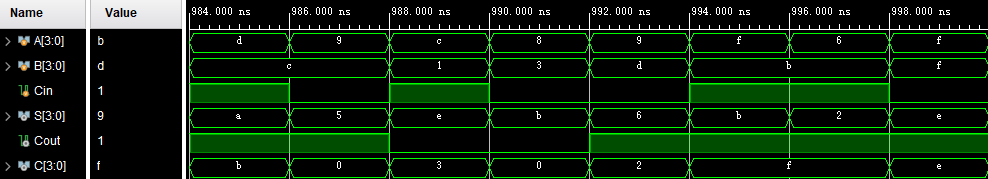
\includegraphics[width=1\textwidth]{4位超前进位加法器波形图.jpg}
            \caption{4位超前进位加法器波形图}
        \end{figure}\par
        \begin{figure}[ht]
            \centering
            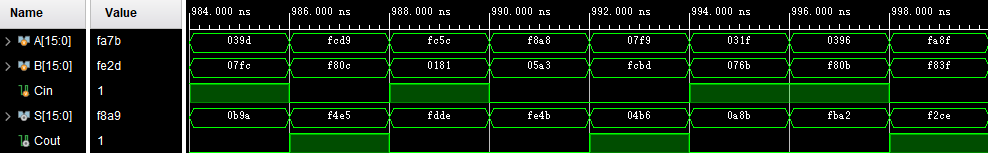
\includegraphics[width=1\textwidth]{16位超前进位加法器.jpg}
            \caption{16位超前进位加法器波形图}
        \end{figure}\par
        \begin{figure}[ht]
            \centering
            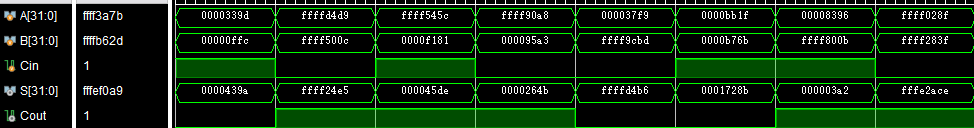
\includegraphics[width=1\textwidth]{32位超前进位加法器波形图.jpg}
            \caption{32位超前进位加法器波形图}
        \end{figure}\par


\section{实验总结}
    \subsection{实例化模块}
        本次实验主要的收获是学会如何实例化模块, 并利用已经写出的模块构建功能更广泛的器件, 另外, 在实例化模块且不需要模块的某些输出时可以不写或者写空括号.
        在器件构建中, 最好自上而下、自下而上两个方向分别考虑, 考虑出结构和接口后进行编写
    \subsection{verilog调试}
        在进行这种多层次结构的程序的调试时, 可以从底层到高层撰写多个testbench来分别进行模拟, 可以更好的进行调试与debug


\section{源代码}
    \subsection{4位数值比较器}
    {\setmainfont{Courier New Bold} 
    \begin{lstlisting}
    module comp_4(
        input [3:0]A,
        input [3:0]B,
        input in_A_G_B,
        input in_A_E_B,
        input in_A_L_B,
        output reg out_A_G_B,
        output reg out_A_E_B,
        output reg out_A_L_B
        );
        wire [3:0]T;
        xnor(T[0],A[0],B[0]);
        xnor(T[1],A[1],B[1]);
        xnor(T[2],A[2],B[2]);
        xnor(T[3],A[3],B[3]);
        
        always @(*)begin
        out_A_G_B = (A[3] & ~B[3]) | 
                    (T[3] & A[2] & ~B[2] ) | 
                    (T[3] & T[2] & A[1] & ~B[1]) | 
                    (T[3] & T[2] & T[1] & A[0] & ~B[0]) | 
                    (T[3] & T[2] & T[1] & T[0] & in_A_G_B);
        out_A_E_B = T[3] & T[2] & T[1] & T[0] & in_A_E_B;
        out_A_L_B = ~(out_A_G_B | out_A_E_B);
        end
        
    endmodule
    \end{lstlisting}}
    \subsection{16位数值比较器}
    {\setmainfont{Courier New Bold} 
    \begin{lstlisting}
    module comp_16(
        input [15:0]A,
        input [15:0]B,
        input in_A_G_B,
        output reg out_A_G_B,
        output reg out_A_E_B,
        output reg out_A_L_B
        );
        wire [3:0]G;
        wire [3:0]E;
        wire [3:0]L;
        
        comp_4 comp0(
            .A(A[3:0]),
            .B(B[3:0]),
            .in_A_G_B(0),
            .in_A_E_B(1),
            .in_A_L_B(0),
            .out_A_G_B(G[0]),
            .out_A_E_B(E[0]),
            .out_A_L_B(L[0])
        );   
        
        comp_4 comp1(
            .A(A[7:4]),
            .B(B[7:4]),
            .in_A_G_B(G[0]),
            .in_A_E_B(E[0]),
            .in_A_L_B(L[0]),
            .out_A_G_B(G[1]),
            .out_A_E_B(E[1]),
            .out_A_L_B(L[1])
        ); 
        
        comp_4 comp2(
            .A(A[11:8]),
            .B(B[11:8]),
            .in_A_G_B(G[1]),
            .in_A_E_B(E[1]),
            .in_A_L_B(L[1]),
            .out_A_G_B(G[2]),
            .out_A_E_B(E[2]),
            .out_A_L_B(L[2])
        ); 
        
        comp_4 comp3(
            .A(A[15:12]),
            .B(B[15:12]),
            .in_A_G_B(G[2]),
            .in_A_E_B(E[2]),
            .in_A_L_B(L[2]),
            .out_A_G_B(G[3]),
            .out_A_E_B(E[3]),
            .out_A_L_B(L[3])
        ); 
        
        always @(*)begin
            out_A_G_B=G[3];
            out_A_E_B=E[3];
            out_A_L_B=L[3];
        end
        
    endmodule
    \end{lstlisting}}
    \subsection{4位超前进位加法器}
    {\setmainfont{Courier New Bold} 
    \begin{lstlisting}
    module add(
        input [3:0]A,
        input [3:0]B,
        input Cin,
        output [3:0]S,
        output [3:0]C,
        output Cout,
        output p,
        output g
        );
        wire [3:0]P;
        wire [3:0]G;
        
        assign P[0] = A[0] ^ B[0];
        assign P[1] = A[1] ^ B[1];
        assign P[2] = A[2] ^ B[2];
        assign P[3] = A[3] ^ B[3];
        
        assign G[0] = A[0] & B[0];
        assign G[1] = A[1] & B[1];
        assign G[2] = A[2] & B[2];
        assign G[3] = A[3] & B[3];
        
        
        assign C[0] = Cin;
        assign C[1] = G[0] | P[0]&Cin;
        assign C[2] = G[1] | (P[1] & (G[0] | (P[0] & Cin)));
        assign C[3] = G[2] | (P[2] & (G[1] | (P[1] & (G[0] | 
                     (P[0] & Cin)))));
        assign Cout = G[3] | (P[3] & (G[2] | 
                     (P[2] & (G[1] | (P[1] & (G[0] | 
                     (P[0] & Cin)))))));
    
            
        assign S[0] = P[0] ^ Cin;
        assign S[1] = P[1] ^ C[1]; 
        assign S[2] = P[2] ^ C[2]; 
        assign S[3] = P[3] ^ C[3]; 
        
        assign p=P[3]&P[2]&P[1]&P[0];
        assign g=G[3] | P[3]&G[2] | P[3]&P[2]&G[1] | 
                 P[3]&P[2]&P[1]&G[0];
        
    endmodule
    \end{lstlisting}}
    \subsection{16位超前进位加法器}
    {\setmainfont{Courier New Bold} 
    \begin{lstlisting}
    module add_16(
        input [15:0]A,
        input [15:0]B,
        input Cin,
        output Cout,
        output [15:0]S,
        output p,
        output g
        );
        wire[3:0]P;
        wire[3:0]G;
        wire[3:0]C;
        wire a;
        wire b;
        
        assign C[0]=Cin;
        
        add pre1(
            .A(A[3:0]),
            .B(B[3:0]),
            .p(P[0]),
            .g(G[0])
        );
        
        add pre2(
            .A(A[7:4]),
            .B(B[7:4]),
            .p(P[1]),
            .g(G[1])
        );
        
        add pre3(
            .A(A[11:8]),
            .B(B[11:8]),
            .p(P[2]),
            .g(G[2])
        );
        
        add pre4(
            .A(A[15:12]),
            .B(B[15:12]),
            .p(P[3]),
            .g(G[3])
        );
        
        add4_inputPG outC(
            .P(P[3:0]),
            .G(G[3:0]),
            .Cin(Cin),
            .C(C[3:0]),
            .Cout()
        );
        
        add add1(
            .A(A[3:0]),
            .B(B[3:0]),
            .Cin(Cin),
            .S(S[3:0]),
            .C(),
            .Cout(),
            .p(),
            .g()
        );
        
        add add2(
            .A(A[7:4]),
            .B(B[7:4]),
            .Cin(C[1]),
            .C(),
            .S(S[7:4]),
            .Cout(),
            .p(),
            .g()
        );
        
        add add3(
            .A(A[11:8]),
            .B(B[11:8]),
            .Cin(C[2]),
            .C(),
            .S(S[11:8]),
            .Cout(),
            .p(),
            .g()        
        );
        
        add add4(
            .A(A[15:12]),
            .B(B[15:12]),
            .Cin(C[3]),
            .C(),
            .S(S[15:12]),
            .Cout(Cout),
            .p(),
            .g()
        );
        
        assign p=P[3]&P[2]&P[1]&P[0];
        assign g=G[3] | P[3]&G[2] | P[3]&P[2]&G[1] | 
                 P[3]&P[2]&P[1]&G[0];
        
    endmodule
    \end{lstlisting}}
    \subsection{32位超前进位加法器}
    {\setmainfont{Courier New Bold} 
    \begin{lstlisting}
    module add32(
        input [31:0]A,
        input [31:0]B,
        input Cin,
        output [31:0]S,
        output Cout
        );
        
        wire [1:0]C;wire p0;wire g0;
        
        assign C[0]=Cin;
        
        add_16 pre(
        .A(A[15:0]),
        .B(B[15:0]),
        .Cin(C[0]),
        .S(),
        .p(p0),
        .g(g0)
        );
        
        assign C[1]=g0 | (p0 & Cin);
        
        add_16 add1(
        .A(A[15:0]),
        .B(B[15:0]),
        .Cin(C[0]),
        .S(S[15:0]),
        .Cout(),
        .p(),
        .g()
        );
        
        add_16 add2(
        .A(A[31:16]),
        .B(B[31:16]),
        .Cin(C[1]),
        .S(S[31:16]),
        .Cout(Cout),
        .p(),
        .g()
        );
        
    endmodule
    \end{lstlisting}}

\end{document}
